\documentclass[sigconf, nonacm]{acmart}
\settopmatter{printfolios=true}
\settopmatter{printacmref=false}
%% PACKAGES
\usepackage{graphicx}
\usepackage{hyperref}
\usepackage{cleveref}
\usepackage{subcaption}
\usepackage{natbib}
\usepackage{mathtools}
\usepackage{xcolor}

%% COLORS
\definecolor{darkgreen}{rgb}{0,0.8,0}

%% TITLES
\title{ALTEGRAD Challenge 2024 on Molecules and NLP: contrastive learning applied to retrieval systems of chemical compounds}

%% AUTHORS
\author{Balthazar Neveu}
\affiliation{%
  \institution{ENS Paris-Saclay}
  \city{Saclay}
  \country{France}
}
\email{balthazar.neveu@ens-paris-saclay.fr}

\author{Léa Khalil}
\affiliation{%
  \institution{Ecole Polytechnique}
  \city{Palaiseau}
  \country{France}
}
\email{leakhalil@yahoo.fr}

\author{Basile Terver}
\affiliation{%
  \institution{Ecole Polytechnique}
  \city{Palaiseau}
  \country{France}
}
\email{terverbasile@mail.com}


%% MAIN DOCUMENT
\begin{document}

  %% KEYWORDS
  \keywords{contrastive learning, graph neural networks, large language models}


  %% Teaser figure
  \begin{teaserfigure}
    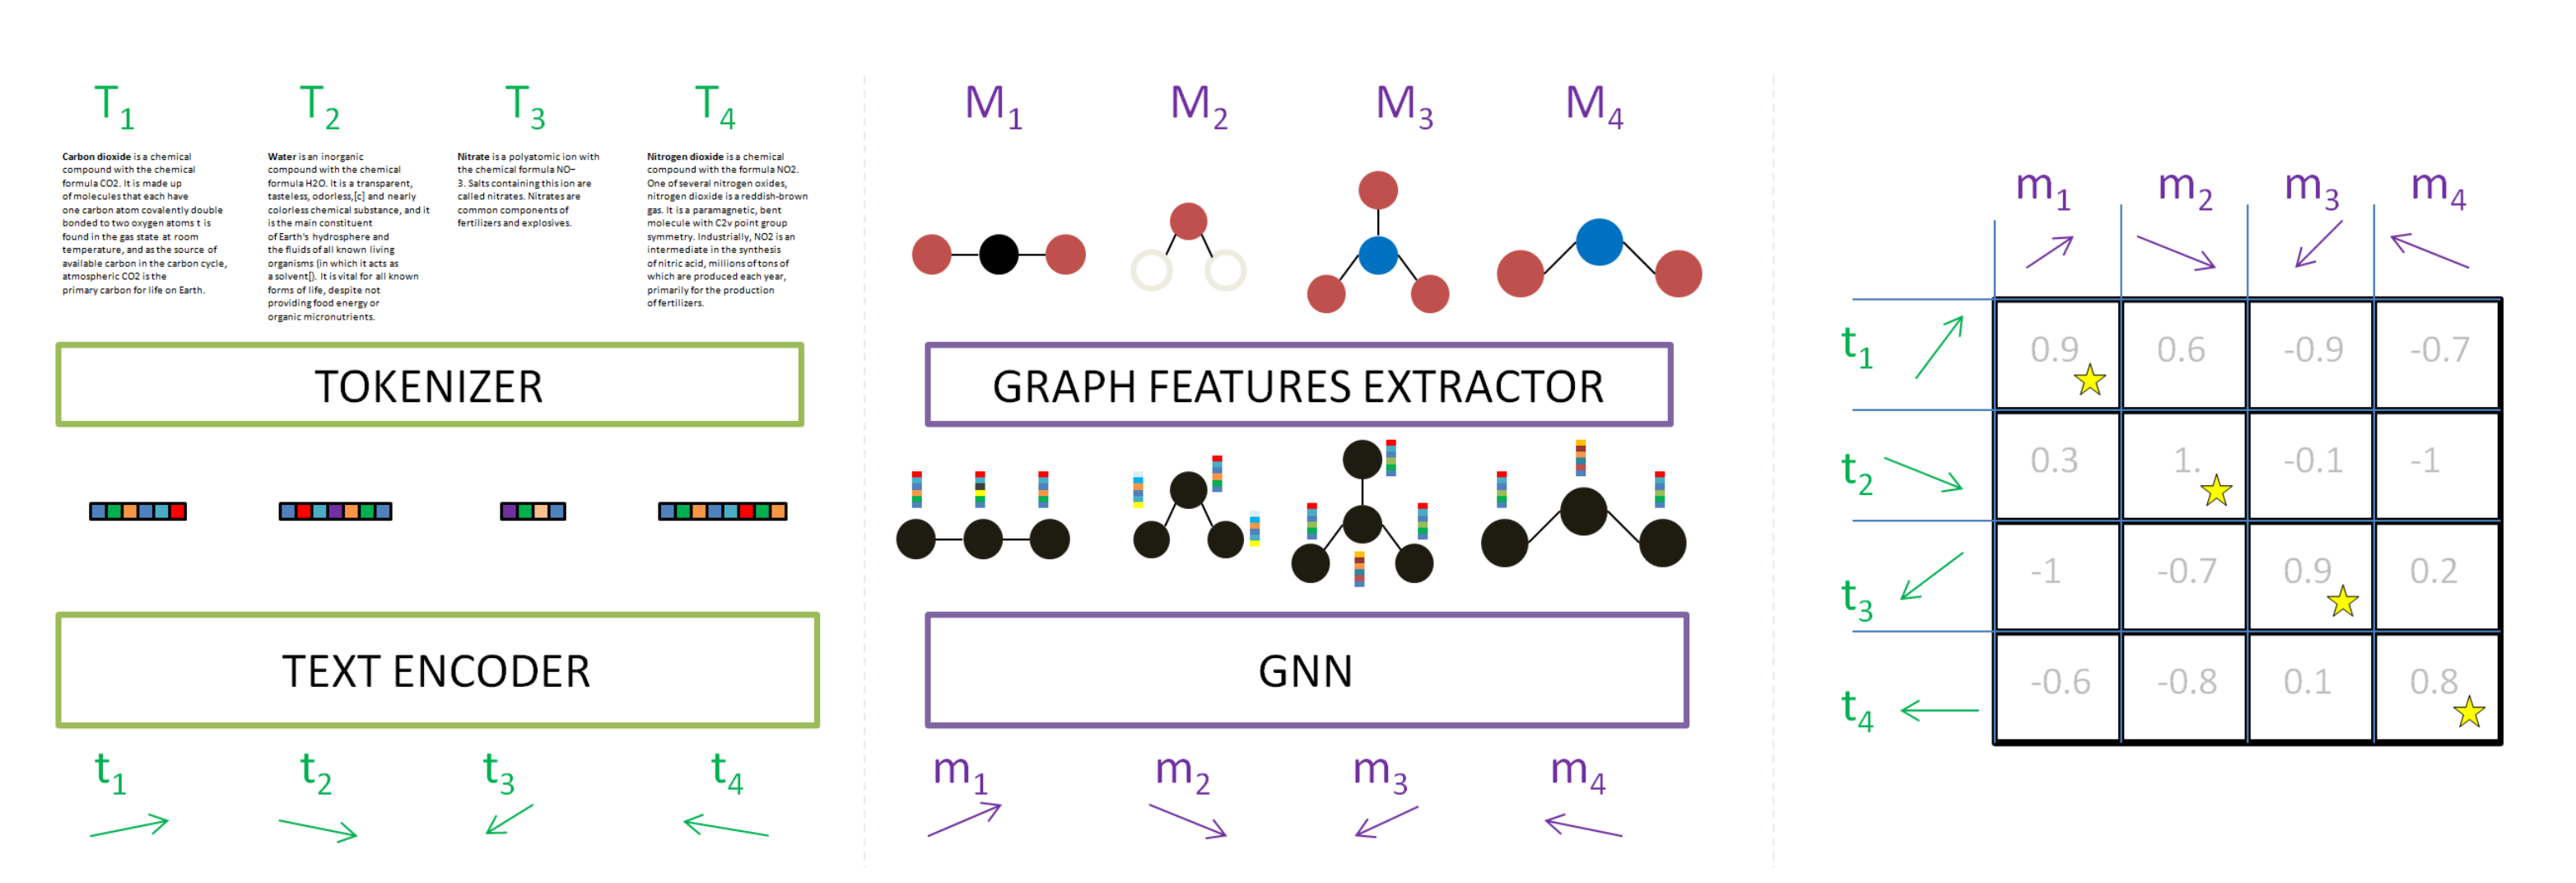
\includegraphics[width=1.\textwidth]{figures/mol_text_overview.PNG}
    \centering
    \caption{On the left side, text descriptions are transformed into sequences of tokens of various lengths. Tokenized sequences are then embedded into a vector space using a language model encoder. Each description $T_{i}$ is transformed into a vector $t_{i}$ (\color{lime} text descriptions embeddings\color{black}). In the middle, molecules $M_{i}$ will be transformed into vector descriptors $m_{i}$ (\color{purple}{molecule embeddings}\color{black}). Each atom is first transformed into a vector using its neighboring atoms. The graph structure is kept as an undirected graphs to model the bounds between atoms. A graph neural network is then used to embed these graphs into a vector space. The molecule and text descriptions embeddings are then compared. At inference time, a text sentence $T$ will be embedded into a vector $t$ which is comparable with relevant matching molecules. The closest molecule embeddings can be proposed to the chemist. Contrastive learning is used to train such a model: supervision comes from the knowlege of the pairing between the molecule and its text description. This is shown on the right side where we compute the similarity between the molecule embedding $m_{i}$ and text embeddings $t_{i}$. The idea behing contrastive learning relies on maximizing similarity between molecules and text embeddings for the correct pair and minimized for the wrong pairs.
    }
    \label{fig:original_pipeline}
  \end{teaserfigure}
  %% TITLE
  \maketitle


  %% ABSTRACT

This study aims at building powerful and consistent vector representions of text descriptions and molecules. The most direct use is a retrieval system for chemical compounds based on text descriptions (good representions can generally also be used for other downstream tasks). Recent advances in contrastive learning allow creating powerful representions for various modalities which can be embedded in a shared vector space. The embedding vectors of both the text description and the molecule shall be similar. We use a pretrained Large Language Model and a Graph Neural Network to create the embeddings. To get an accurate system, complexity mostly comes as an engineering challenge which we had to solve. 

  %% CONTENT
  \section{Introduction}
\label{sec:intro}
Text-2-Mol \cite{text2mol} introduced the groundings of the problem of pairing a text description with the corresponding molecule.
Their contribution also cam with a dataset made of 33k which is always appreciated among the research community.
Here we're using this dataset and the problem is restricted to using this data solely.
We're leveraging the language understanding contained in pretrained Large Language Models (LLM) to create embeddings for text descriptions.
We at least start with models that have good understanding of the English language. The whole point is to transfer this knowledge to the chemical domain to be able to understand molecule structure from a description.
Our code is available on ~\href{https://github.com/balthazarneveu/molecule-retrieval-u sing-nlp}{GitHub}.



  \section{Context}
\label{sec:Context}


\subsection{Dataset}
\label{sec:sota}

\color{red}TODO - Describe dataset in depth and challenge \color{black}


\subsection{State of the art}
\label{sec:sota}

\color{red}TODO - State of the art - Text2mol, CLIP, MolICLR augmentations=Contrastive learning for molecules only\color{black}



\subsubsection{BERT: our base LLM}
\label{sec:bert}
\color{red}TODO - Describe BERT and Distil BERT and SciBERT\color{black}



\subsubsection{GCN: graph convolution networks}
\label{sec:GCN}
\color{red}TODO - Quickly recall Kipf and Welling + using Pytorch geometry (sparse graphs?)\color{black}
  \section{Implementation Strategy}
\label{sec:remplementation}
\subsection*{Methodology}
\label{sec:methodology}
As this work was to  be done in group, we have to develop a framework so everyone could work and share their code independently.
\begin{itemize}
    \item Heterogeneous environments: several operating systems (linux, windows, macOS), various platforms (local laptop training, Kaggle Kernels notebook, remote machines at Ecole Polytechnique). On every platform, data has to be acessible and experiments results have to be stored in a way they can be retrieved. We used the Kaggle dataset feature to  host the raw dataset aswell as the preprocessed data.
    \item Privacy: as not sharing code was among the rules of the challenge, our source code remained private on GitHub (\textit{which made cloning operations even trickier when using Kaggle kernels}).
    \item Reproducibility: all our experiments are reproducible (source code tracking under git, local and cloud storage of experiments results using ~\href{https://wandb.ai/molecule-nlp-altegrad-23/molecule-nlp}{Weights and biases}).
\end{itemize}
An experiment is defined by a unique identifier and the instanciation of a model (tokenization method, architecture of the LLM and GNN), the configuration of an  optimizer and training hyper parameters. At inference time, we're using this unique identifier so we can safely instantiate a network and reload the weights (\textit{trained model are by construction compatible with inference. This avoids the risk of having a `.pth` weight file without knowning which architecture to use to reload it.}).
We wrote a framework which takes and solves all these constraints at once and allows to focus on training models.


\subsection*{Training conditions}
\label{sec:training conditions}
To setup the training loop, we started on a single NVIDIA GeForce RTX 2080 GPU with 6Gb of RAM. This was enough to make sure we could train, track and monitor progress of all our experiments.


\begin{table*}[ht]
    \centering
    \begin{tabular}{lcccc}
    \hline
    \textbf{Feature} & \textbf{Nvidia T500} & \textbf{Nvidia RTX 2060} & \textbf{Nvidia K100} & \textbf{Nvidia A4000} \\ \hline
    Location            & local laptop           & local laptop  & Kaggle  & Ecole Polytechnique  \\
    Access & direct & direct & Kaggle Kernels & SSH \\
    Dataset access & local SSD & local SSD & Kaggle dataset & remote download + SSD drives\\ 
    Memory           & 4 GB                        & 6 GB                           & 16 GB                          & 24 GB                          \\
    \hline
    \end{tabular}
    \caption{Comparison of the GPUs which were used during training}
    \label{table:gpu_comparison}
\end{table*}


\pagebreak

\subsection*{Preliminary study}
\label{sec:preliminary study}

\begin{table*}[h]
    \centering
    \begin{tabular}{|c|c|c|c|c|}
    \hline
    \textbf{Experiment ID} & \textbf{Model Size} & \textbf{LLM} & \textbf{GNN} & \textbf{LRAP} \\ \hline
    101         & 593k                & Frozen Distill-Bert           & Base 3 layer GCN       & 18.7\%      \\ \hline
    106         & 964k                & Frozen Distill-Bert + Adapter & Base 3 layer GCN       & 26.8\%      \\ \hline
    114         & 2.125M              & Frozen Distill-Bert + Adapter & Big 5 layer GCN        & 31.6\%      \\ \hline
    112         & 964k                & Frozen Sci-Bert + Adapter     & Base 3 layer GCN       & 36.7\%      \\ \hline
    113         & 2.125M              & Frozen Sci-Bert + Adapter     & Big 5 layer GCN        & 39.8\%      \\ \hline
    65          & 66.9M               & Trainable Bert                & Base 3 layer GCN       & 63.5\%      \\ \hline
    400         & 110M                & Trainable Sci-Bert            & Base 3 layer GCN       & 66\%        \\ \hline
    \end{tabular}
    \caption{Base Models Specifications and Performances}
    \label{tab:preliminary_study_metrics}
\end{table*}


We start with a few toy experiments to see which architecture factors are most promising (initial hope is that the performances will scale accordingly when we add all extra machine learning tricks).
\textbf{Frozen LLM weights}: We first started with by simple models based on the base GCN (3 graph convolution layers followed by a global pooling layer and 2 layers MLP). Instead of fine tuning all parameters of the LLM, we first started by freezing the LLM parameters. Although simple, this idea intuivitely has many advantages for traing:
\begin{itemize}
    \item We discard the huge memory cost of training a LLM (memory issues not only come from storing the weigths on the GPU but all the optimizers variables during backpropagation). The idea could have been pushed further by pre-computing the text embeddings and storing them on disk. 
    \item Intuivitely, freezing the LLM parameters should make the training more stable as the LLM embeddings acts as a kind of anchor that the GNN shall match.
\end{itemize}
Unfortunately, training achieves low accuracy although the number of parameters to train is lightweight. We added an "adapter" module which is simply a MLP which will adapt by projecting the text representations into a more adapted space which can match with the graph.
\textbf{Influence of the graph neural network size}: We pursued our explorations to see the impact of the GNN size. The \textbf{big GCN} (5 graph convolution layers with 2 residual connection) is more complex and has more parameters to train. We can see that the accuracy is improved by increasing the GCN size. 
\begin{itemize}
    \item Using frozen Distil-BERT: from experiment 106 (base GCN $\text{LRAP}=26.8\%$) to 114 - (big GCN $\text{LRAP}=31.6\%$)
    \item Using frozen SciBERT: from experiment 102 (base GCN $\text{LRAP}=36.7\%$) to 113 - (big GCN $\text{LRAP}=39.8\%$)
\end{itemize}


\textbf{Influence of the pretrained language model}: We also browsed Hugging Face to find models that could be dedicated to scientific-specific language processing. We foud the Sci-Bert\cite{scibert} model and could use it as a drop-in replacement for the Distil-Bert baseline model. Improvements were two-fold when changing the pretrained LLM during this preliminary study: a tokenizer dedicated to a scientific corpus seems by nature a natural choice for scientific words...here atoms and molecule names not being too frequent in common language. The Sci-Bert model may also have reasoning capabilities closer to science and chemistry reactions. This was translated by a improvement in performances. Increasing the GNN size improves accuracy.
\begin{itemize}
    \item Using the Base GCN : from experiment 106 Distil-BERT ($\text{LRAP}=26.8\%$) to experiment 112 - SciBert ($\text{LRAP}=36.7\%$).
    \item Using the Big-GCN: from experiment 114 Distil-BERT ($\text{LRAP}=31.6\%$) to experiment 113 - SciBert ($\text{LRAP}=39.8\%$).
\end{itemize}
The capacity of the network (same number of parameters) being fixed between these two experiments, it proves that the SciBERT tokenization and pretraining is definitely more suited for our task. We'd hope that this $seq 8\%$ LRAP improvement would be translated when training a fully trainable LLM.

Unfortunately we later conducted larger experiments with fully trainable LLM (starting from the pretrained weights) and the performances differences were not as good as expected. Using the Base GCN : from experiment 65 Distil-BERT ($\text{LRAP}=63.5\%$) to experiment 400 - SciBert ($\text{LRAP}=66\%$), there's not that $seq 8\%$ LRAP improvement that we had seen earler. Furthermore, it's hard to tell whether the 2.5\% improvement is due to the SciBert model pretraining being more suited for our task or the fact that the model has nearly twice as many trainable parameters than the Distil-BERT. 

This preliminary study gave us guidance that using a larger GCN and using SciBERT pretrained weights and tokenizer were good trends to follow to try improving our results. The pitfall is that fine tuning SciBERT comes with a bigger memory footprint than Distil-BERT which requires diminishing batch sizes for a fixed GPU (and as stated in the CLIP paper, large batch size seems to be one key factor of the success of contrastive learning). Experiments 65 and 400 have been cautiousy trained with batches of size 32 and same hyperparameters to get comparable results: 
\begin{itemize}
    \item the SciBERT experiment 400 was only possible using a NVIDIA RTX A4000 with 24Gb of RAM \item the Distil-BERT experiment 65 was possible on a NVIDIA Tesla T100 with 16Gb of RAM (Kaggle Kernels notebook).
\end{itemize}



\begin{figure*}[ht]
    \centering
    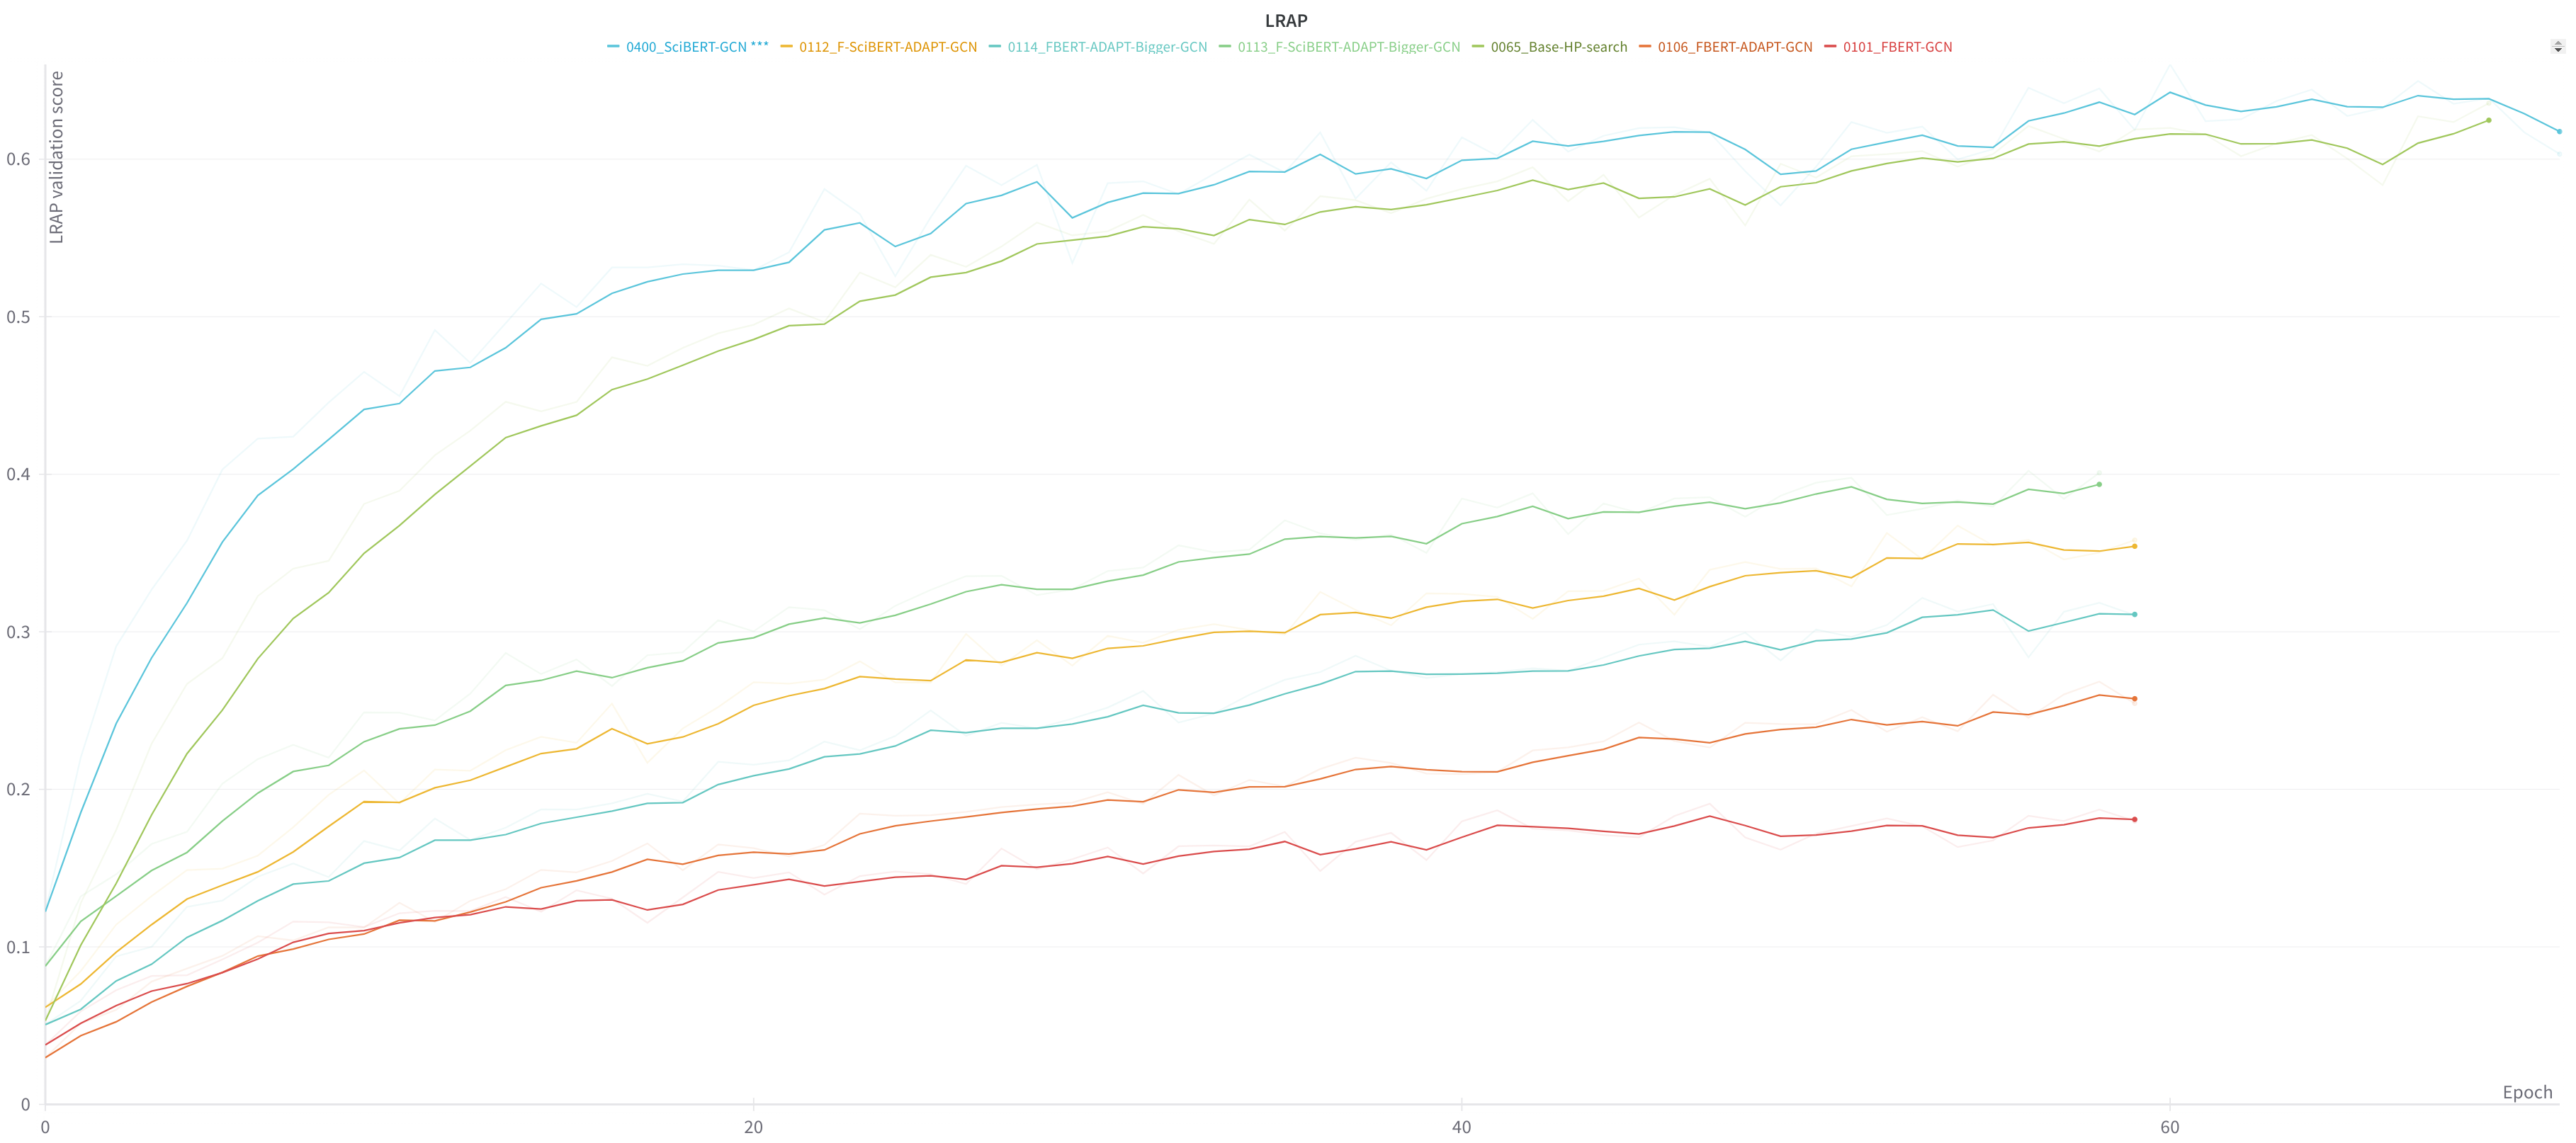
\includegraphics[width=1.\textwidth]{figures/preliminary_study.png}
    \caption{Training curves for the preliminary study.}
    \label{fig:preliminary_study_curves}
\end{figure*}


  \section{Discussion on the Paper}
\label{sec:discussion}
Discussion
  \section{Conclusion}
\label{sec:conclusion}

In conclusion...


  \newpage

  %% APPENDIX
  \appendix
  \section{Appendix}
Appendix
  
  \newpage
  %% BIBLIOGRAPHY
  \bibliographystyle{ACM-Reference-Format}
  \bibliography{references}

\end{document}
